\subsubsection{Gegentaktschaltung} \label{subsec:gegentakt}

In der realen Stromverteilung wird beabsichtigt, dass der Stromfluss über einen Zuleiter zum Verbraucher hinein-, respektive über einen Ableiter herausgeführt wird. 
Diese Art der Signalübertragung wird als Gegentakt-Betrieb bezeichnet. Im realen Stromnetz ist allerdings auch der sogenannte Gleichtakt-Betrieb vorhanden. Dabei wirken alle Leiter als Zuleiter, der Gesamte Strom wird durch die Erde weggeleitet. Durch das Gesetz der Superposition ist es möglich, den Gleichtakt- und den Gegentaktanteil getrennt voneinander zu betrachten. Dieses Phänomen wird Anhand der Abbildung \ref{fig:auftrennen_der_leitung} klar. 

\begin{figure}[H]
	\centering
	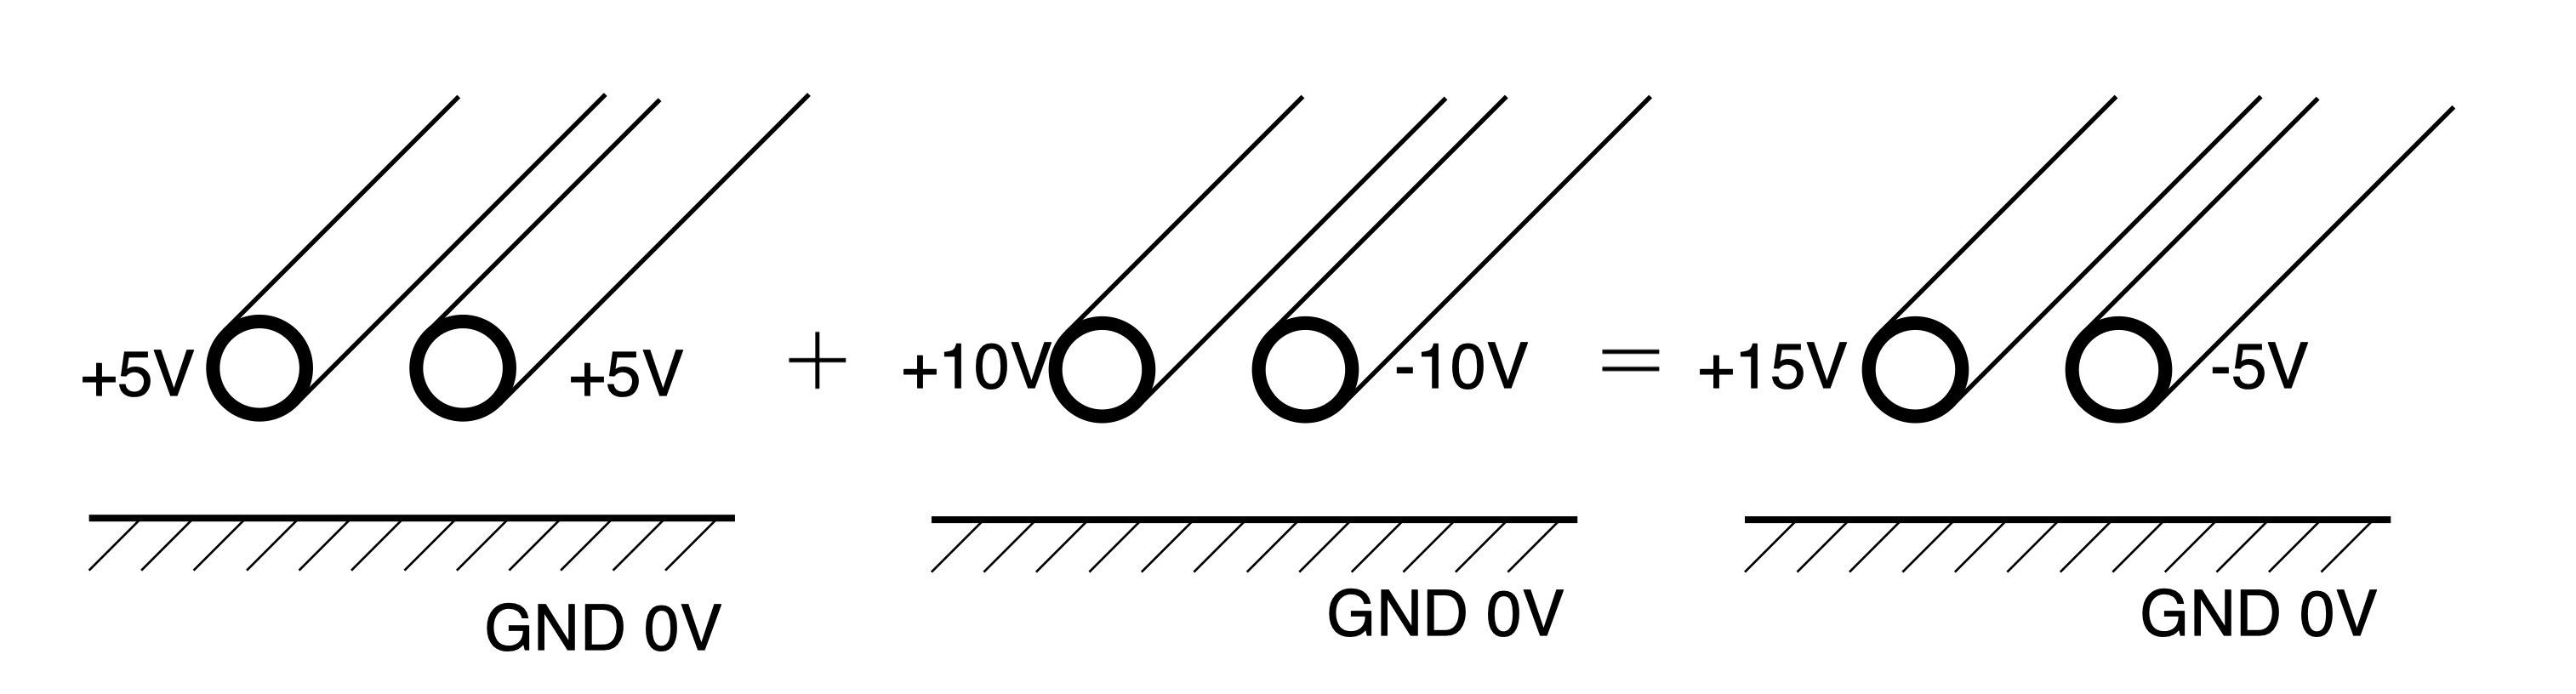
\includegraphics[width=15cm]{grundsatz_cm_dm.jpg}
	\caption{Beispiel der aufgetrennten Leitung}
	\label{fig:auftrennen_der_leitung}
\end{figure} 


An einen geerdeten Verbraucher sind 2 Phasen angeschlossen. An der Zuleitung liegt eine Spannung von 15 Volt an, an der Rückleitung liegen -5 Volt an. Diese Leitung wird nun aufgeteilt in eine Gleichtaktleitung, bei welcher über beide Phasen 5 Volt eingespeist werden und in eine Gegentaktleitung, in welcher durch die Zuleitung 10 Volt, respektive in der Rückleitung -10V eingespiesen werden. Während in der Gleichtaktleitung die Addierten 10 Volt gegenüber der Erde anliegen, werden sie in der Gegentaktleitung abgeführt.



